\documentclass{beamer}
\mode<presentation>
\usetheme{CambridgeUS}
\usepackage[russian]{babel}
\usepackage[utf8]{inputenc}
\usepackage[T2A]{fontenc}
\usepackage{sansmathaccent}

\usepackage{verbatim}
\usepackage{alltt}

\pdfmapfile{+sansmathaccent.map}
\title[Software Design]{Паттерн Шаблонный метод}
\author{Наумов Д.А., доц. каф. КТ}
\date[03.12.2019] {Основы программной инженерии, 2019}

\begin{document}

%ТИТУЛЬНЫЙ СЛАЙД
\begin{frame}
  \titlepage
\end{frame}
  
\section{Паттерн Шаблонный метод}

\begin{frame}
\begin{figure}[h]
\centering
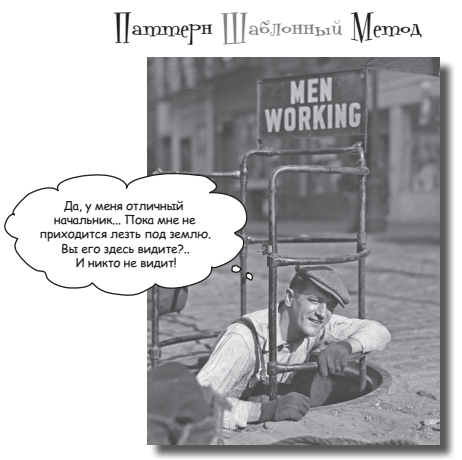
\includegraphics[scale=0.6]{images/lec12-pic01.png}
\label{pic-sort}
\end{figure}
\end{frame}

\begin{frame}
\begin{figure}[h]
\centering
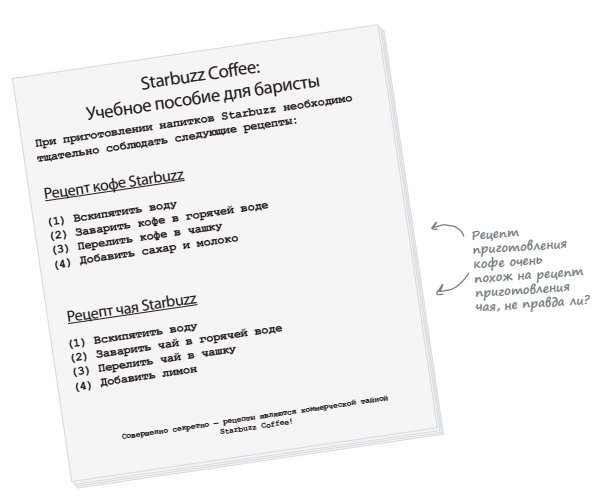
\includegraphics[scale=0.6]{images/lec12-pic02.png}
\label{pic-sort}
\end{figure}
\end{frame}

\begin{frame}
\begin{figure}[h]
\centering
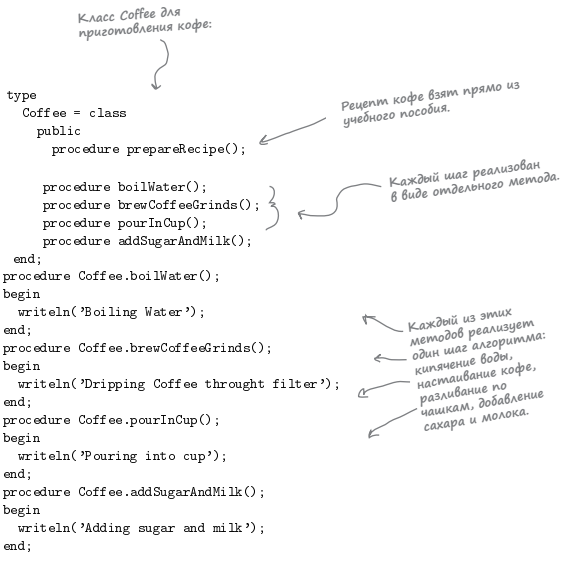
\includegraphics[scale=0.6]{images/lec12-pic03.png}
\label{pic-sort}
\end{figure}
\end{frame}

\begin{frame}
\begin{figure}[h]
\centering
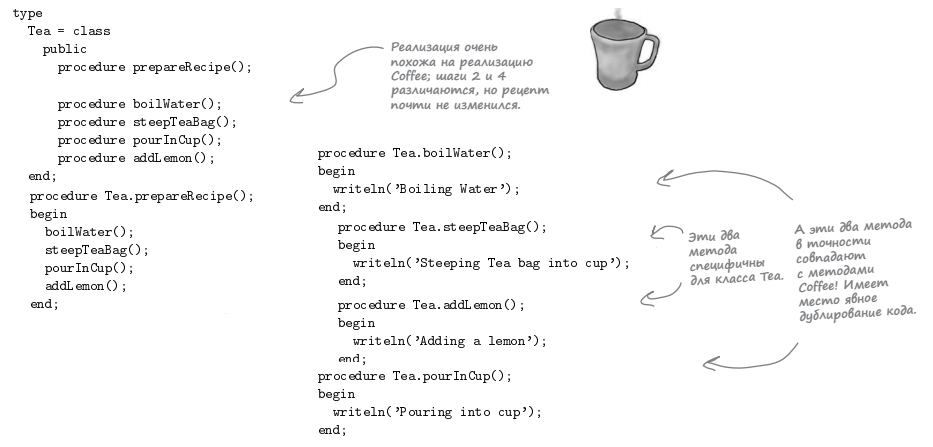
\includegraphics[scale=0.5]{images/lec12-pic04.png}
\label{pic-sort}
\end{figure}
\end{frame}

\begin{frame}
\begin{figure}[h]
\centering
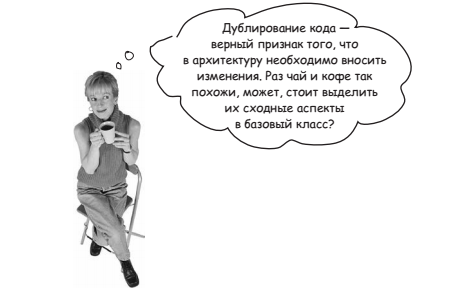
\includegraphics[scale=1.0]{images/lec12-pic05.png}
\label{pic-sort}
\end{figure}
\end{frame}

\begin{frame}
\begin{figure}[h]
\centering
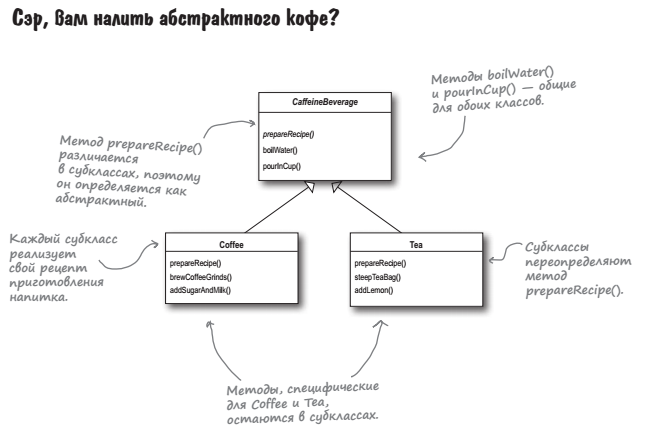
\includegraphics[scale=0.6]{images/lec12-pic06.png}
\label{pic-sort}
\end{figure}
\end{frame}

\begin{frame}
\begin{figure}[h]
\centering
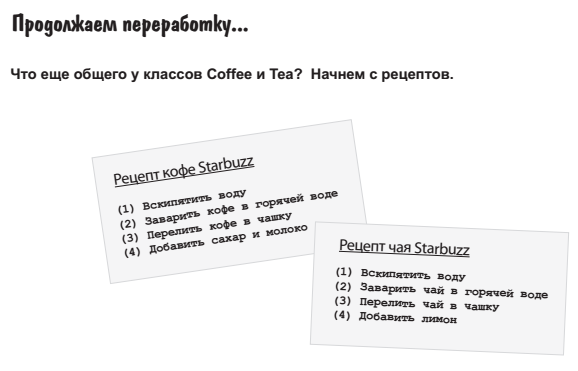
\includegraphics[scale=0.6]{images/lec12-pic07.png}
\label{pic-sort}
\end{figure}
\end{frame}

\begin{frame}
\begin{figure}[h]
\centering
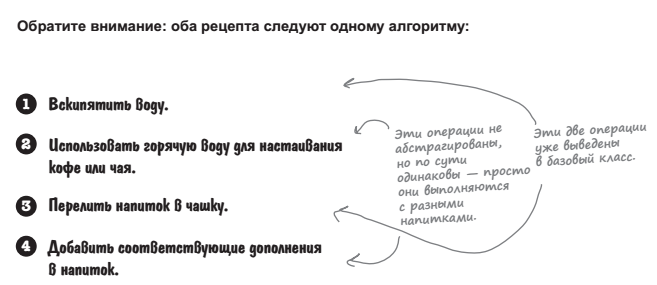
\includegraphics[scale=0.6]{images/lec12-pic08.png}
\label{pic-sort}
\end{figure}
\end{frame}

\begin{frame}
\begin{figure}[h]
\centering
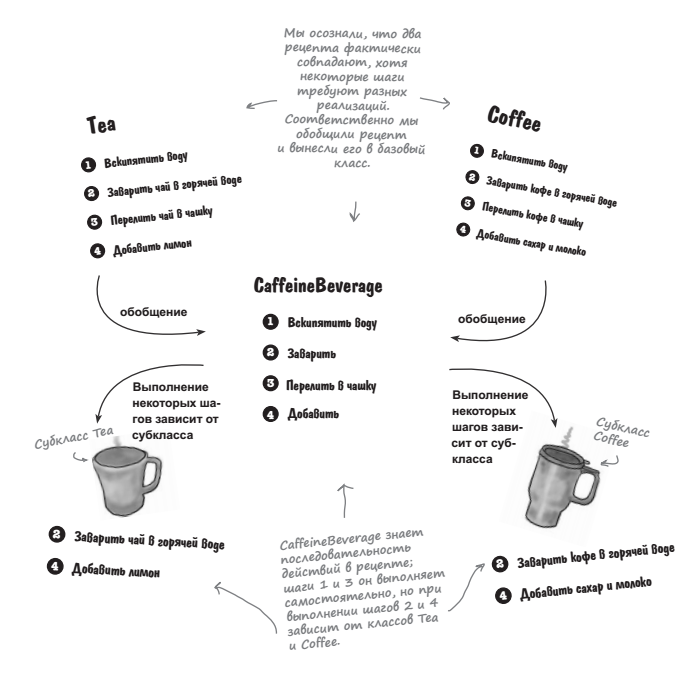
\includegraphics[scale=0.6]{images/lec12-pic09.png}
\label{pic-sort}
\end{figure}
\end{frame}

\begin{frame}
\begin{figure}[h]
\centering
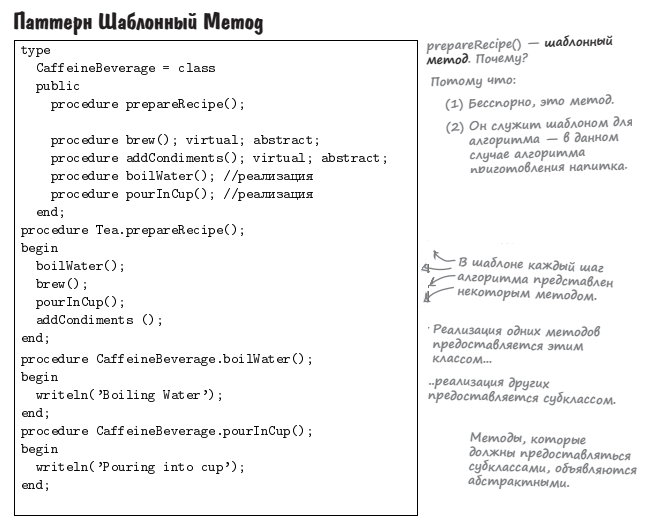
\includegraphics[scale=0.5]{images/lec12-pic10.png}
\label{pic-sort}
\end{figure}
\end{frame}

\begin{frame}
\begin{figure}[h]
\centering
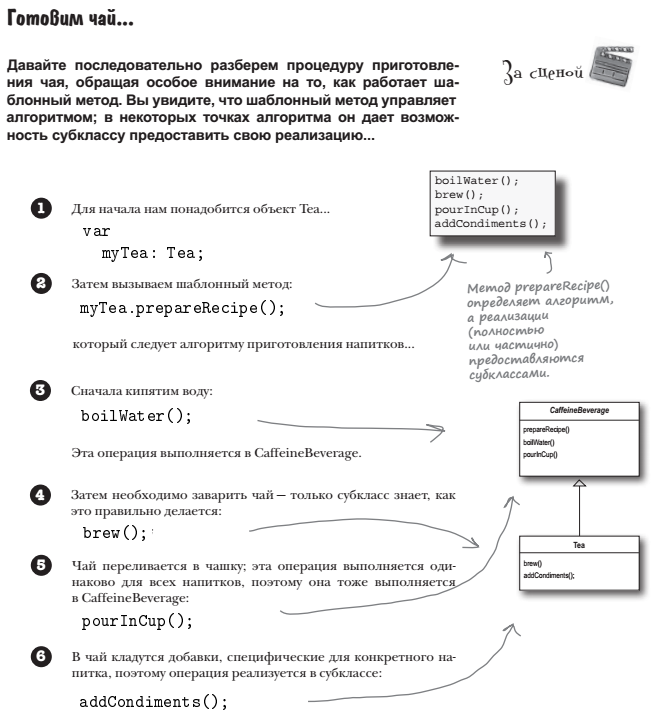
\includegraphics[scale=0.45]{images/lec12-pic11.png}
\label{pic-sort}
\end{figure}
\end{frame}

\begin{frame}
\begin{figure}[h]
\centering
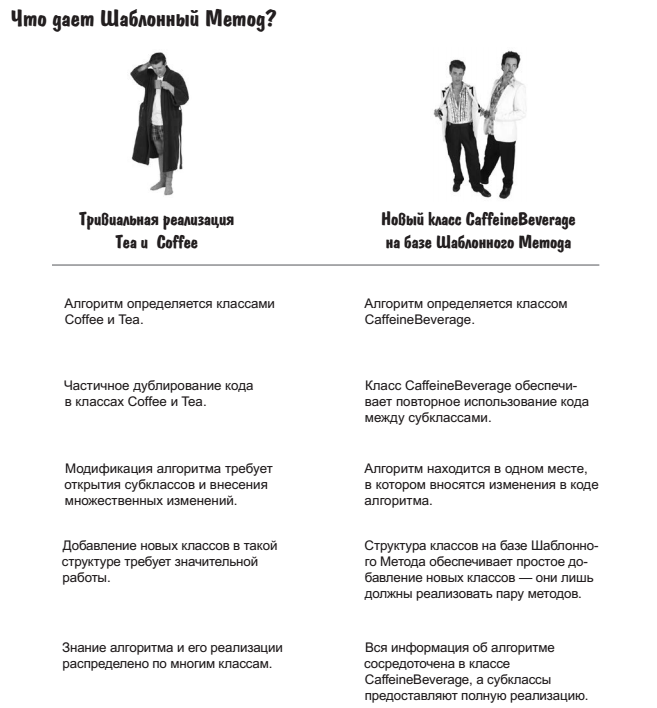
\includegraphics[scale=0.5]{images/lec12-pic12.png}
\label{pic-sort}
\end{figure}
\end{frame}

\begin{frame}
\begin{figure}[h]
\centering
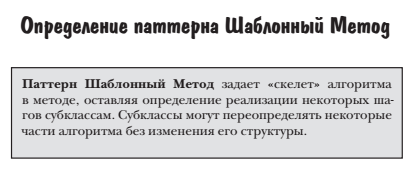
\includegraphics[scale=0.8]{images/lec12-pic13.png}
\label{pic-sort}
\end{figure}
\end{frame}

\begin{frame}
\begin{figure}[h]
\centering
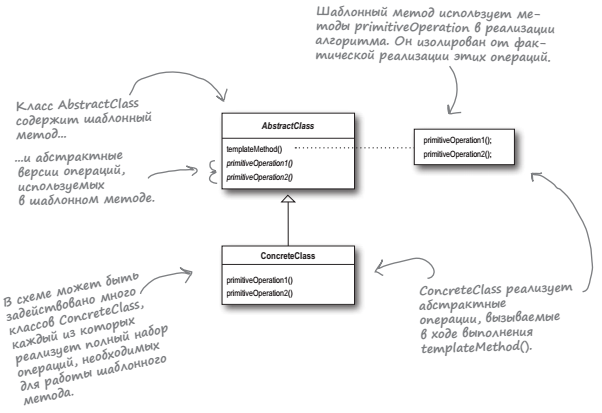
\includegraphics[scale=0.7]{images/lec12-pic14.png}
\label{pic-sort}
\end{figure}
\end{frame}

\begin{frame}
\begin{figure}[h]
\centering
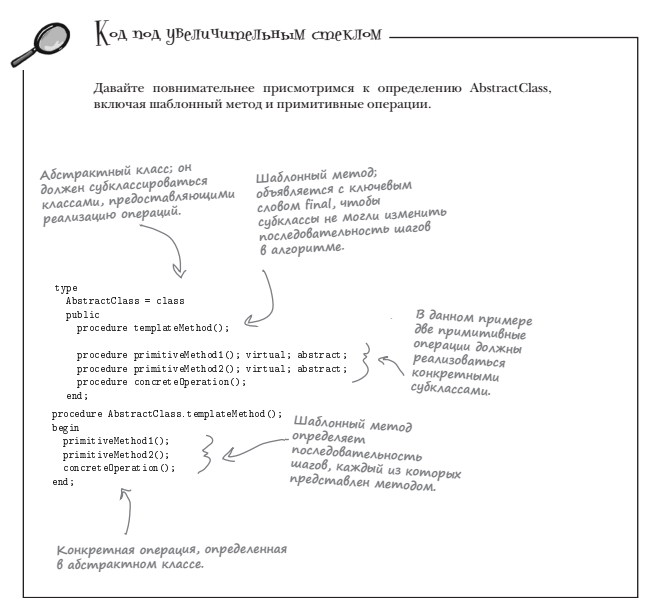
\includegraphics[scale=0.5]{images/lec12-pic15.png}
\label{pic-sort}
\end{figure}
\end{frame}

\begin{frame}
\begin{figure}[h]
\centering
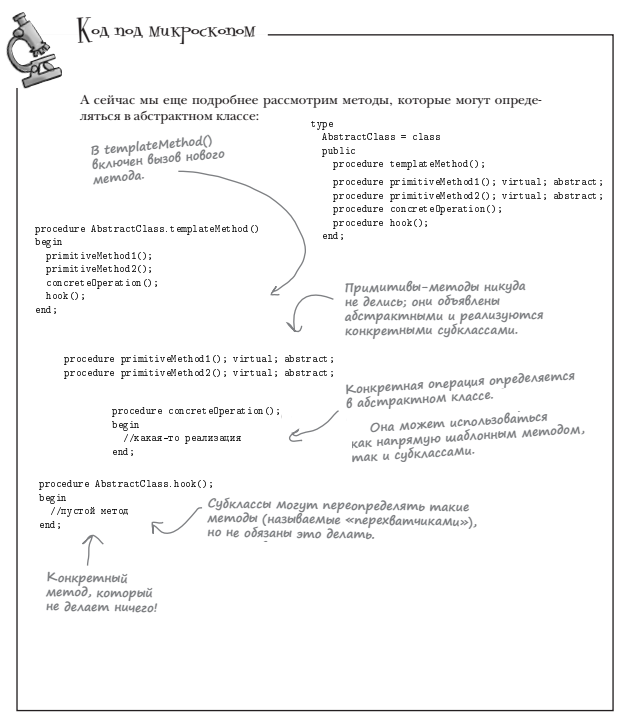
\includegraphics[scale=0.5]{images/lec12-pic16.png}
\label{pic-sort}
\end{figure}
\end{frame}

\begin{frame}
\begin{figure}[h]
\centering
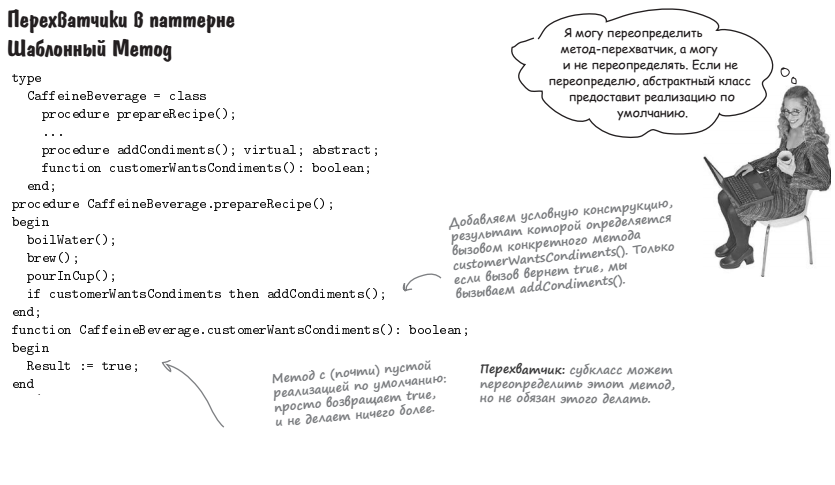
\includegraphics[scale=0.5]{images/lec12-pic17.png}
\label{pic-sort}
\end{figure}
\end{frame}

\begin{frame}
\begin{figure}[h]
\centering
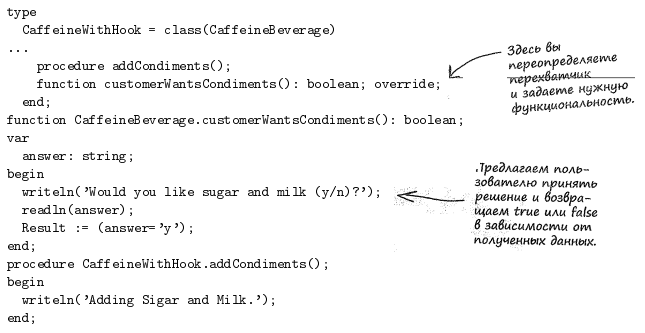
\includegraphics[scale=0.6]{images/lec12-pic18.png}
\label{pic-sort}
\end{figure}
\end{frame}

\end{document}